

%!TEX root = ../thesis.tex
%******************************************************************************
\chapter[Conceptual Framework]{A Conceptual Framework for High-Performance Near-Time Processing of Bulk Data}\label{ch:conceptual_framework}

%******************************************************************************
\todo[inline]{Alternative title: A Conceptual Framework for Feedback-Controlled Computer Systems}

\section{Introduction} 
\begin{figure}
	[htpb] \centering 
	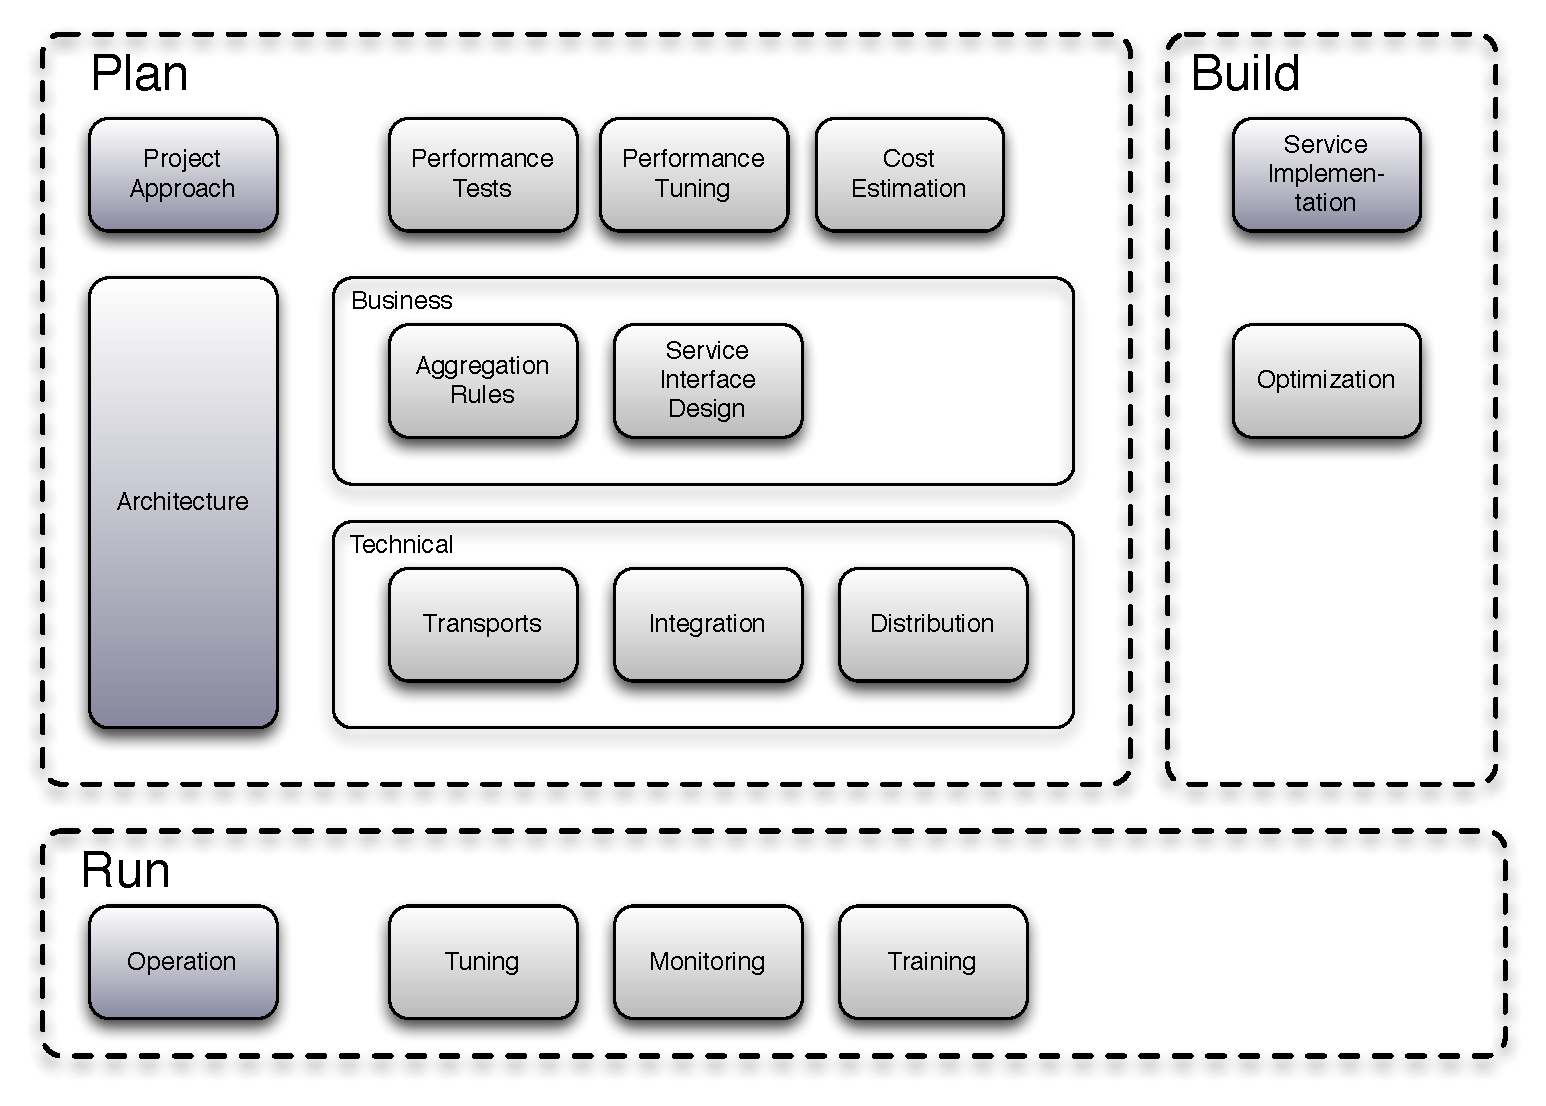
\includegraphics[width=\textwidth]{ch6_conceptual_framework_overview} \caption{Overview of Conceptual Framework} \label{fig:ch6_conceptional_framework_overview} 
\end{figure}

\section{Metamodel} 
\begin{itemize}
	\item View
	\item Role
	\item Task
	\item Deliverable
\end{itemize}

\begin{figure}
	[htpb] \centering 
	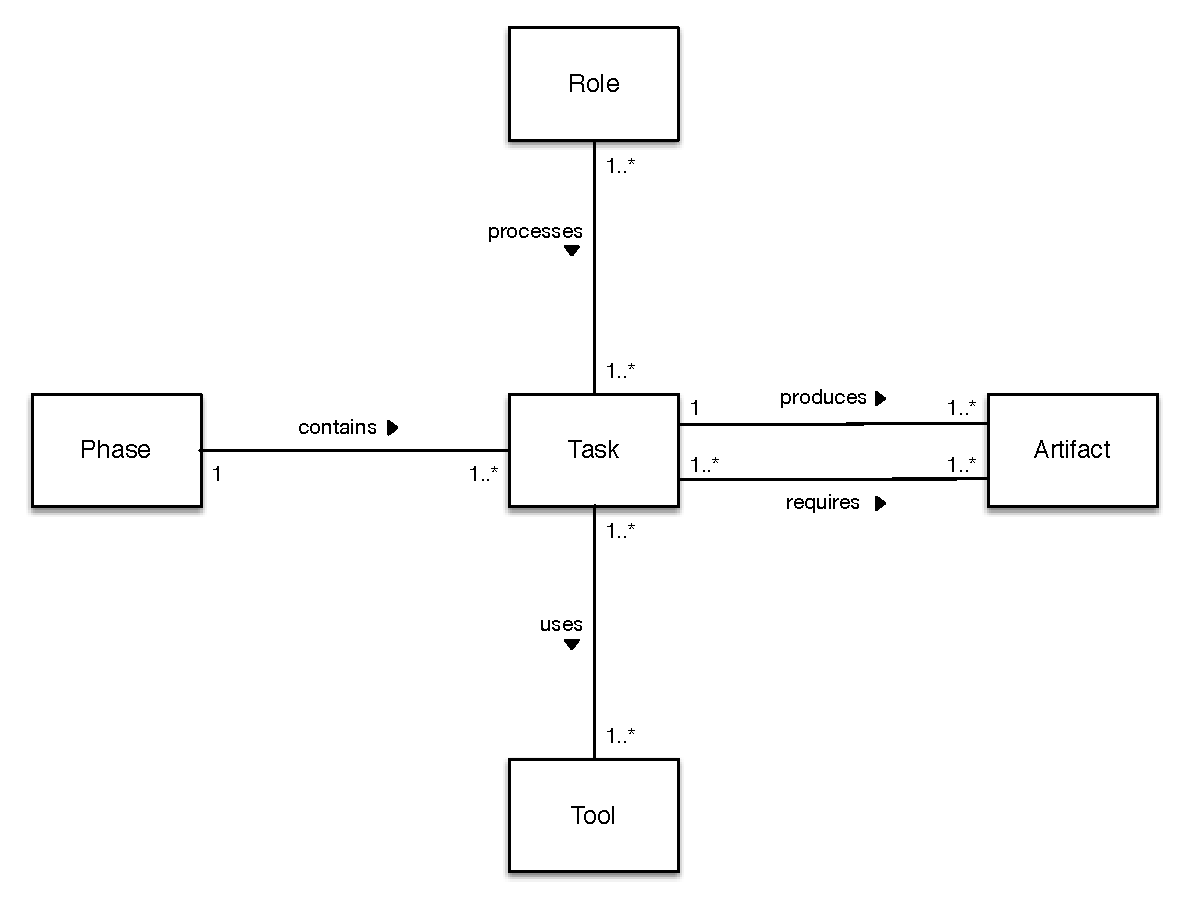
\includegraphics[width=\textwidth]{ch6_metamodel} 
	\caption{Metamodel} 
	\label{fig:ch6_metamodel} 
\end{figure}

\section{Views}
\begin{itemize}
	\item Plan
	\item Build
	\item Run
\end{itemize}

\section{Roles} 
\begin{itemize}
	\item System Architect 
	\item Business Analyst 
	\item Developer 
	\item Tester 
	\item Project Manager 
	\item Operations Engineer 
	\item Service Architect 
	\item Service Developer
\end{itemize}

\subsection{System Architect} 
\begin{table}
	[h!] \caption{System Architect} \label{table:ch6_Role_System_Architect} \centering 
	\begin{tabular}
		{|m{2cm}|m{10cm}|} \hline \bfseries Role & System Architect\\
		\hline \bfseries Description & Lorem ipsum\\
		\hline \bfseries Tasks & 
		\begin{itemize}
			\item Define System Architecture 
		\end{itemize}
		\\
		\hline \bfseries Artifacts & System Architecture\\
		\hline 
	\end{tabular}
\end{table}

\section{Processes/Tasks} 
\begin{itemize}
	\item Define System Architecture 
	\item Define Integration Architecture
	\begin{itemize}
		\item Transports
		\item Distribution
	\end{itemize}
	\item Define Controller Architecture 
	\begin{itemize}
		\item Define Control Problem 
		\item Define Input/Output Variables 
	\end{itemize}
	\item Perform Controller Tuning 
	\begin{itemize}
		\item System Model/System Identification 
		\item Static Tests
		\item Step Tests
	\end{itemize}
	\item Define Service Interfaces 
	\item Define Aggregation Rules 
	\item Define Performance Tests 
	\item Setup Monitoring infrastructure
	\item Setup Test and Integration Environment
	\item Deploy to Test and Integration Environment
	\item Perform Performance Tests
\end{itemize}
\begin{table}
	[h!] \caption{Define System Architecture} \label{table:ch6_Task_Define_System_Architect} \centering 
	\begin{tabular}
		{|m{3cm}|m{10cm}|} \hline \bfseries What & Define System Architecture\\
		\hline \bfseries Why & Lorem ipsum\\
		\hline \bfseries Who & System Architect\\
		\hline \bfseries Artifacts & System Architecture\\
		\hline \bfseries Challenges & Lorem Ipsum\\
		\hline \bfseries Best practises & Lorem ipsum\\
		\hline 
	\end{tabular}
\end{table}

\section{Building Blocks/Artifacts}

\section{Reference Architecture}

\section{Related Work}

\section{Summary} 
